% 本原稿用の条件マクロ
%章ごとにコンパイルできるようにするための設定.
%このマクロが定義されていない場合,チャプター内は個別のTEXソースとして扱われる.
\expandafter\ifx\csname MasterFile\endcsname\relax
\documentclass[a4j,twoside,12pt,dvipdfmx]{thesis} % 修論・卒論など (ページが右端にでる) 
\usepackage{amsmath, amssymb}
\usepackage{mysettings}
\usepackage{graphicx}
\usepackage{color}
\usepackage{comment}

\begin{document}

\addtocounter{chapter}{+1}

\setlength{\baselineskip}{1.95zw}
\setlength{\textheight}{30\baselineskip}
\mainmatter

\fi
% これより上は削除しちゃダメ
% 本原稿用の条件マクロここまで
%
%\newcommand{\argmax}{\mathop{\rm arg~max}\limits}
\newcommand{\argminnnn}{\mathop{\rm arg~min}\limits}
\renewcommand\thefootnote{\arabic{footnote})}
\def\vector#1{\mbox{\boldmath $#1$}}

\chapter{関連研究}\label{rel}
% ここに本文
本章では,本研究で取り扱っている基礎知識について説明する.本章の構成は次の通りである.\ref{rel:preKnowledge}節では前提知識について述べる. \ref{rel:GNN}節ではグラフニューラルネットワークについて述べる.

\section{前提知識}\label{rel:preKnowledge}
本節では, 研究を行うにあたって必要な前提知識について述べる.
\subsection{fastText}
fastText\cite{bojanowski2017enriching}は Facebook AI Research によって開発された自然言語処理ライブラリである.このライブラリを使用することで,単語埋め込みの生成やテキストの分類ができる.
\subsection{Transductive, Inductive}
本項ではTransductive, Inductiveの2つの言葉の意味について説明をする.
Transductiveな学習とは, 学習時にデータは存在するもののラベルが割り振られていないデータに対してラベル付けを行う学習であり, グラフニューラルネットワークでは一般的な,学習時にすべてのノードを必要とする学習である.
\par それに比べてInductiveな学習とは, 学習時に存在しなかったデータに対しての推論を行う学習である. Inductiveな学習を行うグラフニューラルネットワークモデルには,次節で登場するGraphSAGEが該当する.


\section{グラフニューラルネットワーク}\label{rel:GNN}
本節では, グラフニューラルネットワーク (GNN) に関する歴史や関連研究について述べる.
\subsection{GNNの歴史}
1997年にSperdutiら\cite{sperduti1997supervised}により, ニューラルネットワーク上で初めてグラフ構造が扱われた. この研究は初期のGNNの先駆的な研究となった.その後, Goriet ら\cite{gori2005anew},  Scarselli ら \cite{scarselli2009the} , Gallicchio ら \cite{gallicchio2010graph} によりGNNに関する研究が行われてきた.
これらの研究はRNNのアーキテクチャを用いてグラフのノード埋め込みを学習することを目的としている. 周辺ノードの情報伝播を同じ関数を用いて再帰的に行い, すべてのノードの埋め込みが平衡状態になるまで伝播を続ける. この周辺ノードの情報伝播の概念は, GCNに受け継がれている.

\subsection{Graph Convolutional Network}
Graph Convolutional Network (GCN) \cite{kipf2017semi} は,CNN のような畳み込み演算を GNN に適用したモデルである.1 層の GCN を用いるとそれぞれのノードが隣接するノードの情報を畳み込むという特徴がある.
隣接行列 $A$ と特徴行列 $X$ を GCN に与える入力とすると,GCN の第$l$層における出力は式\ref{eq:GCN}で表される.
\begin{equation}
  \label{eq:GCN}
  H^{(l)}=f(\tilde{D}^{-\frac{1}{2}}\tilde{A}\tilde{D}^{-\frac{1}{2}}H^{(l-1)}W_{1}^{(l-1)})
\end{equation}
ここで,$\tilde{A} = A + I_{N}$はノード自身へのエッジを追加した無向グラフの隣接行列であり,$I_N$は単位行列である.
$\tilde{D}_{ii} = \sum_{j} \tilde{A}_{ij}$であり,$W_{1}^{(l)}$は層に応じた学習可能な重み行列,$f(\cdot)$は$ReLU(\cdot) = \max (0, \cdot)$のような活性化関数である.
また,$H^{(0)}=X$となる.\par
GCN は層の数を増やしすぎると,全てのノードの埋め込みが同じ値に収束してしまい,性能が低下することがわかっている.

\subsection{GraphSAGE}
GraphSAGEはGCNを拡張したものであり, Inductiveな学習を行うことができるモデルである. GCNとの違いとして, GraphSAGEでは近傍ノードをサンプリングし, それを集約するためのaggregate関数を学習を学習する. GraphSAGEでの前方伝播方法は図\ref{fig:SAGE}に示す.
\begin{figure}
  \centering
  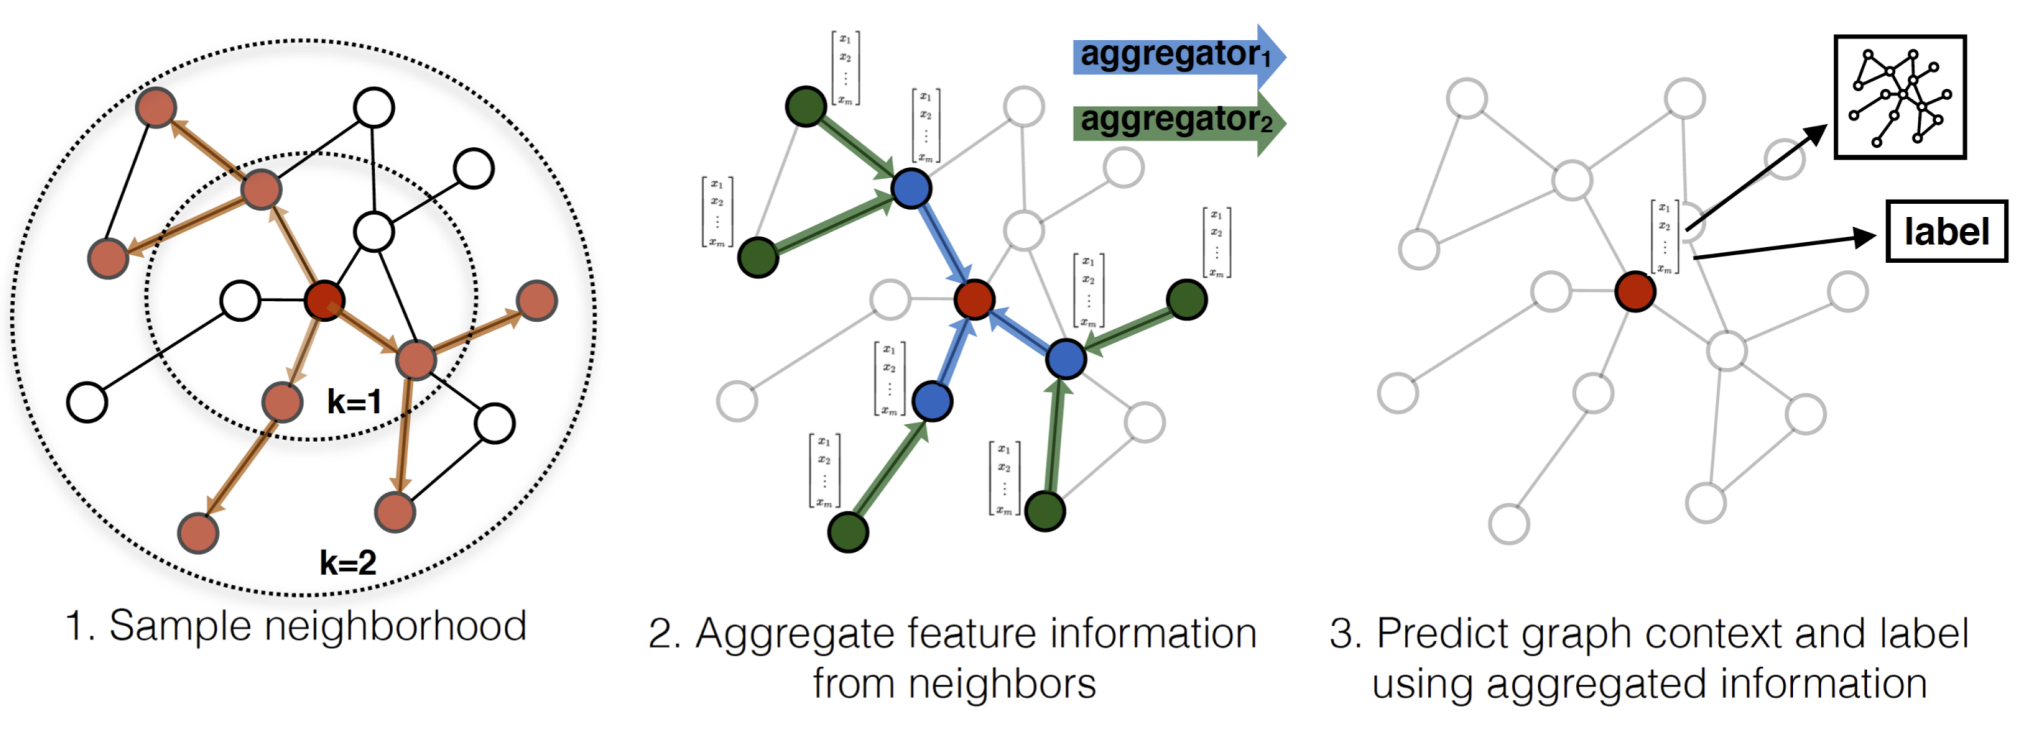
\includegraphics[width=\linewidth]
  {img/GraphSAGE.png}
  \caption{GraphSAGEの前方伝播 (\cite{hamilton2017inductive}より引用)}
  \label{fig:SAGE}
\end{figure}

aggregate関数のアーキテクチャには3種類が存在する.
\subsubsection{Mean aggregator}
Mean aggregatorを用いた場合, ノード$v$に対するGraphSAGEの第$l$層の出力は式\ref{eq:MeanAgg}で表される.
\begin{equation}
  \label{eq:MeanAgg}
  h_{v}^{l} \leftarrow \sigma(\mathbf{W_{2}} \cdot \mathrm{MEAN} (\{ \mathbf{h}_{v}^{l-1}\} \cup \{ \mathbf{h}_{u}^{l-1} , \forall u \in \mathcal{N}(v) \}))
\end{equation}
ここで, $\mathbf{h}_{v}^{l}$は第$l$層でのノード$v$の埋め込みであり, $\mathbf{W_{2}}$は学習可能な重み行列, $\mathcal{N}(v)$はノード$v$の近傍ノード郡である.
このアーキテクチャはGCNと同様の処理をInductiveな学習に対応させたものである.

\subsubsection{LSTM aggregator}
LSTM アーキテクチャに基づく, より複雑なaggregator. Mean aggregator に比べて, LSTM aggregator は表現力に優れている. しかし, LSTMは入力を逐次的に処理するため, ノードの入力順に応じて結果が変化する. そのため, ノードの近傍を不規則に並び替えることで, 非順序集合でLSTMを動作させた.

\subsubsection{Pooling aggregator}
Pooling aggregatorは, 近傍ノードを全結合層に与え, その結果の中で最大となるものを選択する.これは, 式\ref{eq:PoolAgg}で表される.
\begin{equation}
  \label{eq:PoolAgg}
  \mathrm{AGGREGATE}_{k}^{\mathrm{pool}} = \max(\{ \sigma ( \mathbf{W_{2}}_{pool} \mathbf{h}_{u_{i}}^{k} + \mathbf{b} ), \forall u_{i} \in \mathcal{N}(v) \})
\end{equation}
ここで, $\sigma$ は非線形の活性化関数であり, $\mathbf{b}$はバイアスである.

\subsection{SimGNN}
SimGNN\cite{bai2019simgnn}はGNNを用いて近似的に Graph Edit Distance(GED)を求めるモデルである.グラフの入力ノードにはラベルが割り振られており,ノードの特徴量はラベルの One-Hot ベクトルとなる.
この手法では,入力グラフを複数層の GCN に与えることでノードレベルの埋め込みを生成した後,以下に示すアテンションモジュールを元にグラフレベルの埋め込みを生成する.
それらの非線形の変換をし, global graph context $c \in \mathbb{R}^{D}$を得る.
\begin{equation}c = \tanh (\frac{1}{N}W_{3}{\displaystyle \sum_{n=1}^{N}} u_{n})\end{equation}
ここで,$u_{n} \in \mathbb{R}^{D}$は入力ノード$n$の埋め込み,$D$はノードの埋め込みの次元,$W_{3} \in \mathbb{R}^{D \times D}$は学習可能な重み行列である.
$c$は重み行列を学習することで,グラフの全体的な構造及び特徴量を表すことができ,これに基づいて各ノードの重要度を計算することが可能となる.\par
ノード$n$に対しての重要度$a_{n}$の計算は,ノード$n$の埋め込み$u_{n}$と$c$の内積を計算した後,シグモイド関数$\sigma(x) = \frac{1}{1+exp(-x)}$を用いることで,重要度$a_{n}$を$(0,1)$の範囲に収める.
ここではグラフサイズを埋め込みに反映するため,全体の重要度を正規化しない.
重要度を計算した後,グラフレベルの埋め込み$h \in \mathbb{R}^{D}$を重み付きのノードの埋め込みの総和$h = \sum_{n=1}^{N}a_{n}u_{n}$で計算する.
アテンションモジュールについてまとめると式\ref{eq:Att}になる.
\begin{equation}
  \label{eq:Att}
  h = \sum_{n=1}^{N}\sigma(u_{n}^\mathsf{T}c)u_{n}= \sum_{n=1}^{N}\sigma(u_{n}^\mathsf{T} \tanh (\frac{1}{N}W_{3}\sum_{m=1}^{N}u_{m}))u_{n}
\end{equation}
AttentionModule から 2 つのグラフの埋め込み$h_{i} \in \mathbb{R}^{D}, h_{j} \in \mathbb{R}^{D}$が与えられた後,
それらの関係をモデル化するために,式\ref{eq:NTN} で表されるニューラルテンソルネットワークを用いる.
\begin{equation}
  \label{eq:NTN}
  g(h_{i}, h_{j})=f(h_{i}^\mathsf{T}W_{4}^{[1:K]}h_{j} + V \begin{bmatrix} h_{i}\\h_{j} \end{bmatrix} + b)
\end{equation}

ここで,$W_{4}^{[1:K]} \in R^{D \times D \times K}$は重み行列,$\begin{bmatrix} $ $ \end{bmatrix}$は結合操作,$V \in \mathbb{R}^{K\times2D}$は重みベクトル.
$b \in \mathbb{R}^{K}$はバイアスベクトル,$f(\cdot)$は$ReLU(\cdot) = \max (0, \cdot)$のような活性化関数である.
$K$は K は各グラフ埋め込みペアに対してモデルが生成する類似度の数を制御するハイパーパラメータである.\par


\subsection{Self-Attention Graph Pooling (SAGPool)}
Self-Attention Graph Pooling (SAGPool) \cite{lee2019self} はグラフプーリング手法の一つである. SAGPool を用いることでSelf-Attentionに基づいたノードの削減を行うことができる. この手法では, ノードの重要度は式\ref{eq:SAScore}で示される.
\begin{equation}
  \label{eq:SAScore}
  Z = \sigma (\tilde{D}^{-\frac{1}{2}}\tilde{A}\tilde{D}^{-\frac{1}{2}}X\Theta_{att})
\end{equation}
ここで, $\tilde{A} = A + I_{N}$はノード自身へのエッジを追加した無向グラフの隣接行列であり,$I_N$は単位行列である.
$\tilde{D}_{ii} = \sum_{j} \tilde{A}_{ij}$であり$\Theta_{att}$はSAGPool層のパラメータである.
GCNを用いることで, グラフの特徴と構造情報の両方に基づいた重要度を得ることができる.
ノードの重要度を元に, Gao ら\cite{gao2019proceedings} によるノード選択方法を行うことで, 上位$\lceil kN \rceil$個のノードを保持する.ここで,$k \in (0,1)$はプーリングの割合である. 式\ref{eq:topk}はノード選択法を表す.
\begin{equation}
  \label{eq:topk}
  \mathrm{idx} = \textrm{top-rank}(Z, \lceil kN \rceil ), Z_{mask} = Z_{\mathrm{idx}}
\end{equation}
ここで, $\textrm{top-rank}$ は上位$\lceil kN \rceil$個のノードを返し, $\cdot_{\mathrm{idx}}$は$\mathrm{idx}$が示すノードのみの重要度である.
最終的に, 式\ref{eq:SAGPool}に表すように, 上位$\lceil kN \rceil$個のノードのみのグラフを作成する.
\begin{equation}
  \label{eq:SAGPool}
  X' = X_{\mathrm{idx},:}, X_{out} = X' \odot Z_{mask}, A_{out} = A_{\mathrm{idx,idx}}
\end{equation}
ここで, $X_{\mathrm{idx},:}$は$\mathrm{idx}$が示すノードの特徴量行列であり, $\odot$ はアダマール積 (要素ごとの積) であり, $A_{\mathrm{idx,idx}}$は$\mathrm{idx}$が示すノードの隣接行列である.

% 本原稿用の条件マクロ
% これ以降は削除しちゃダメ
\expandafter\ifx\csname MasterFile\endcsname\relax
\def\MasterFile{本原稿です}

% 参考文献
%% 本原稿用の条件マクロ
%章ごとにコンパイルできるようにするための設定.
%このマクロが定義されていない場合,チャプター内は個別のTEXソースとして扱われる.
\expandafter\ifx\csname MasterFile\endcsname\relax
\documentclass[a4j,12pt]{thesis} % 修論・卒論など (ページが右端にでる)   
\usepackage{mysettings}
\usepackage{url}

\begin{document}

\setlength{\baselineskip}{1.95zw}
\setlength{\textheight}{30\baselineskip}
\backmatter

\fi
% これより上は削除しちゃダメ
% 本原稿用の条件マクロここまで

%参考文献

\bibliographystyle{junsrt}
\bibliography{thesisB}

\clearpage


% 本原稿用の条件マクロ
% これ以降は削除しちゃダメ
\expandafter\ifx\csname MasterFile\endcsname\relax
\def\MasterFile{本原稿です}
\end{document}
\fi
% 本原稿用の条件マクロここまで


\bibliographystyle{junsrt}
\bibliography{thesisB}

\end{document}
\fi
% 本原稿用の条件マクロここまで
